\chapter{Computed Tomography (CT)}

Computed Tomography (CT) is a medical imaging modality that became
clinically available in the early 1970s and was the first to be made
possible by computers. CT can provide isotropic\footnote{Isotropic
  spatial resolution is a characteristic of images where the
  resolution is equal in all directions. In the case of 3D images,
  this means that a voxel (a 3D pixel) is a perfect cube, with equal
  dimensions on all sides.: along the X-axis (left-right), the Y-axis
  (up-down), and the Z-axis (front-back). } 3D images (volumes),
including axial\footnote{An axial view divides the body horizontally
  into a top (superior) and bottom (inferior) section.},
coronal\footnote{A coronal view divides the body vertically into a
  front (anterior) and back (posterior) section.}, and
sagittal\footnote{A sagittal view divides the body vertically into a
  right and left section.} views. The images are obtained by X-ray
transmission, moving an X-ray tube (the gantry, see
Figure~\ref{fig:CT_equipment_machine}) and detector arrays around the
patient(see Figure~\ref{fig:views_in_CT}).

\begin{figure}
  \centering
    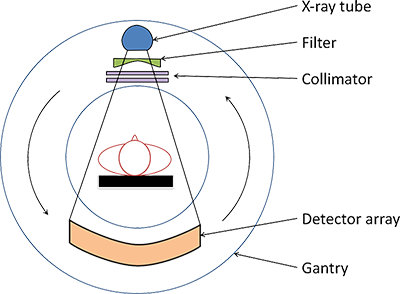
\includegraphics{CT_equipment_machine}
  \caption{ \cite{morin2025radiation}.\label{fig:CT_equipment_machine}}
\end{figure}

\begin{figure}
  \centering
  \begin{tabular}{cc}
    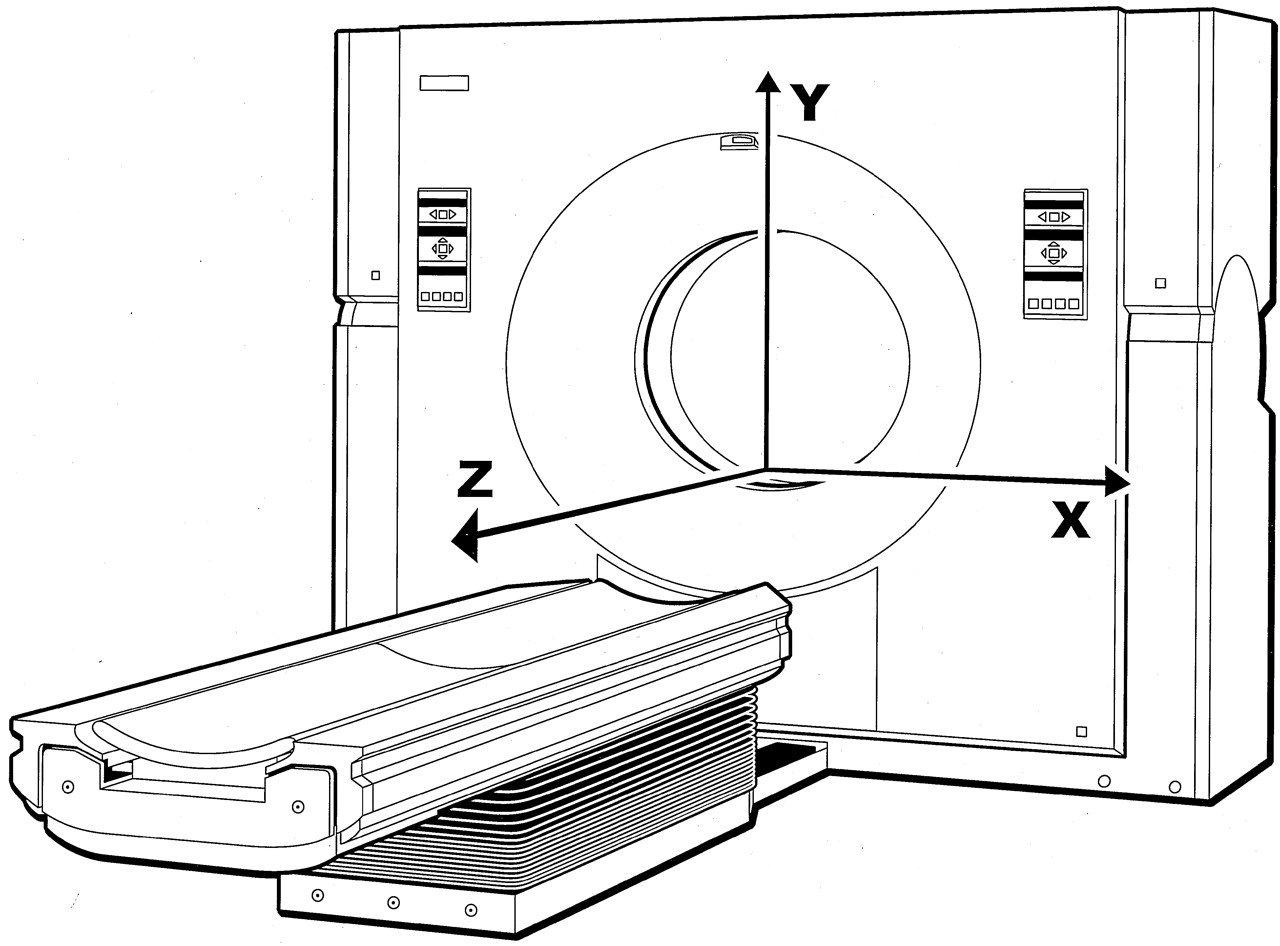
\includegraphics{CT_axis} & 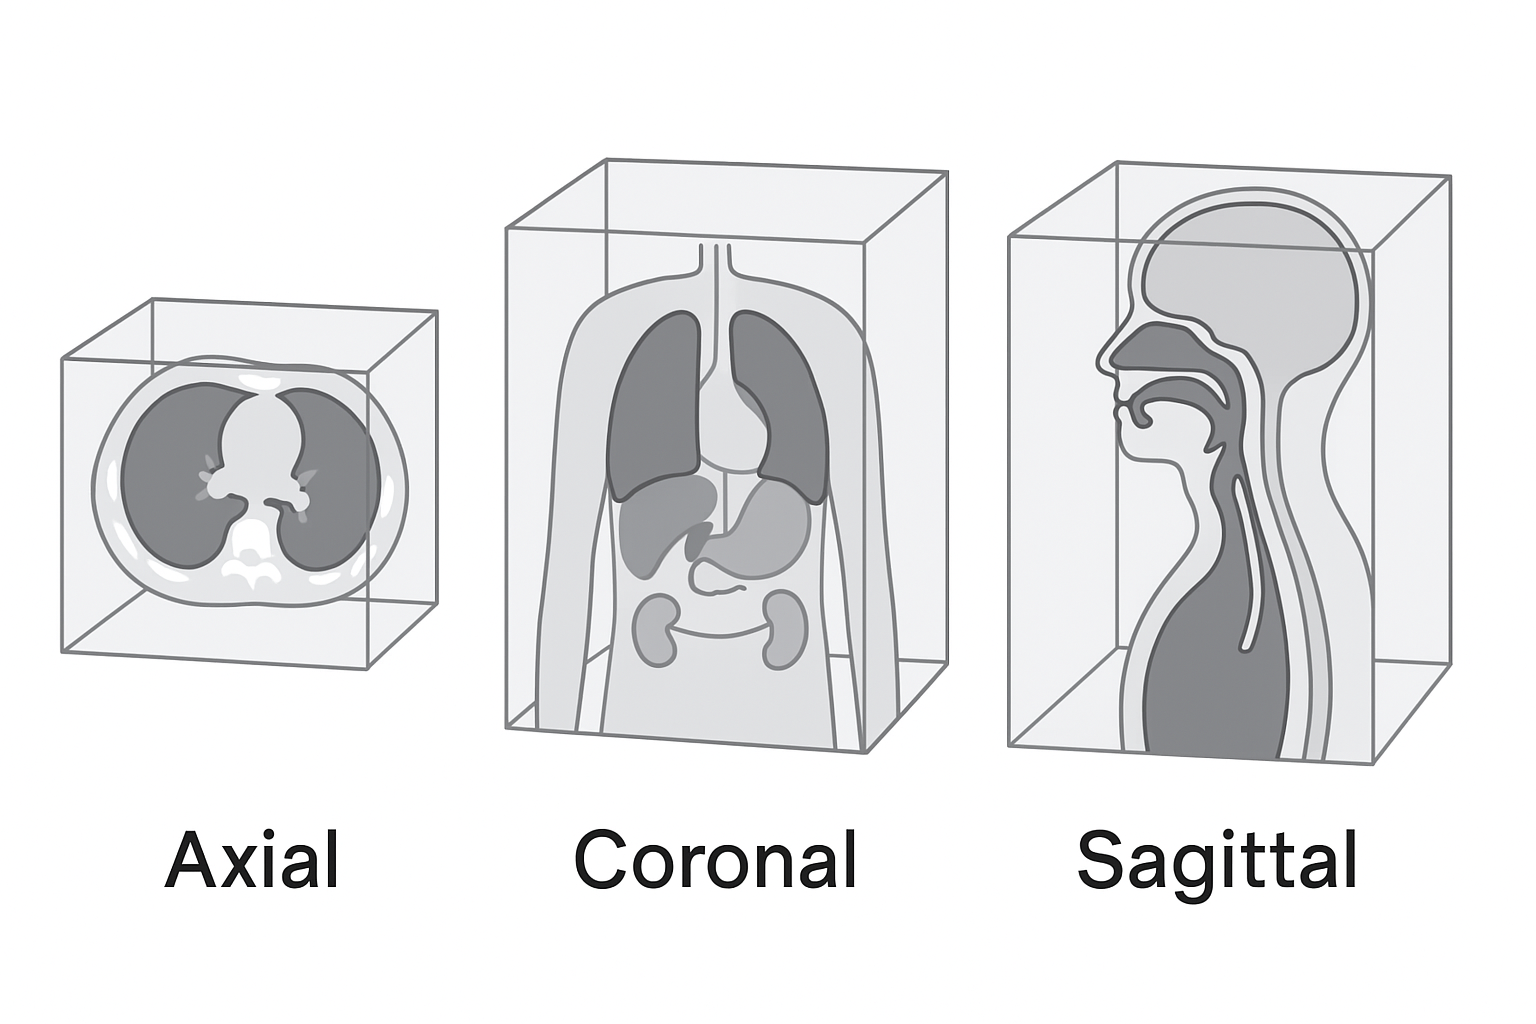
\includegraphics{axial_coronal_sagittal}
  \end{tabular}
  \caption{Reference axis used in CT and type of views generated \cite{morin2025radiation}.\label{fig:views_in_CT}}
\end{figure}

While CT is usually used for anatomic imaging, the use of
iodinated contrast injected intravenously allows the functional
assessment of various organs as well \cite{bushberg2011essential}.

\section{Acquisition}

\begin{figure}
  \centering
  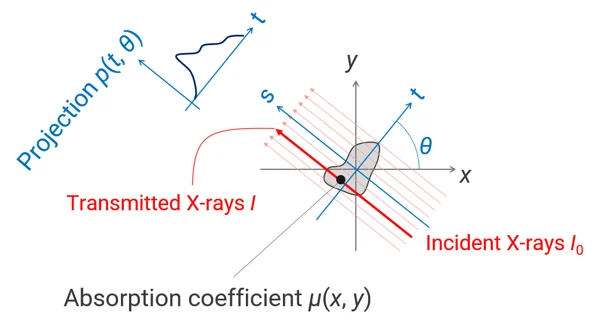
\includegraphics{projection}
  \caption{A projection example \cite{takase2025CT}. $\theta$ is the
    angle used for taking the projection and $t$ the location in
    the detector.\label{fig:projection}}
\end{figure}

The 2D data collected from each angle is called a \emph{projection}
(see Figure~\ref{fig:projection}), consisting of multiple individual
attenuation measurements. The acquisition process can be classified as
(see Figure~\ref{fig:CT_geometries}):

\begin{figure}
  \centering
  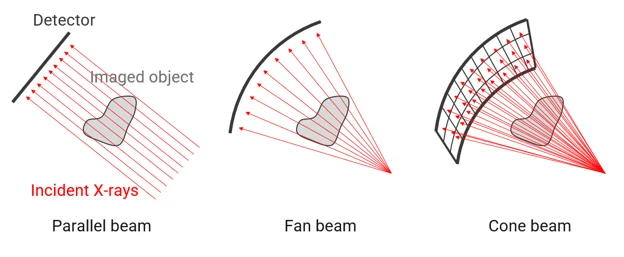
\includegraphics{CT_geometries}
  \caption{Geometries used in CT \cite{takase2025CT}.\label{fig:CT_geometries}}
\end{figure}

\begin{enumerate}
\item \textbf{Parallel-beam acquisition}: The X-rays are parallel
  (usually using a collimator) and the detector is organized as a 1D
  array.

\item \textbf{Fan-beam acquisition}: The X-rays form a fan with the vertice in the emitter
  in a line (using a collimator) and the detector is organized as a 1D
  array.

\item \textbf{Cone-beam acquisition}: The X-rays form a cone with the
  vertice in the emitter, and the detector is a 2D array.
  
\end{enumerate}

\begin{figure}
  \centering
  \begin{tabular}{cc}
    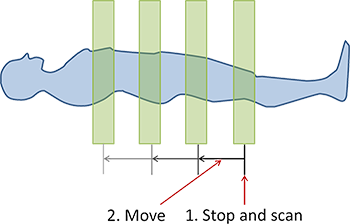
\includegraphics{axial_scanning} & 
\includegraphics{helical_scanning}
  \end{tabular}
  \caption{Types of scanning used in CT \cite{abdulla2025acquiring1}.\label{fig:scannings}}
\end{figure}

Depending on how the scanning is performed, we can distinguish between
(see Figure~\ref{fig:scannings}):

\begin{enumerate}
\item \textbf{Axial (sequential) scanning}:
  The gantry completes a 360-degree rotation to acquire projection
  data while the patient table is stationary. 

\item \textbf{Helical (spiral) scanning}: The patient table moves
  at a constant speed while the gantry rotates, causing the X-rays
  source to form a helix around the patient.
\end{enumerate}

\section{Image reconstruction}
The CT scaner generates a collection (usually thousands) of
projections that need to be processed to obtain the 3D
reconstruction. In parallel- and fan-beam scaners, the projections are
(1D) lines and the set of all projections for the same Z-plane form a
2D image called \emph{sinogram}
\cite{wikipedia2025radom_transform}\footnote{The Radon transform
  describes how CT projections are mathematically related to the
  scanned object; back-projection is the reconstruction method that
  (with filtering) approximates the inverse Radon transform to recover
  the object from its projections.}. In cone-beam scaners, the
sinogram is a 3D cube.

To generate the 3D reconstruction, the following tasks are usually done:

\begin{figure}
  \centering
  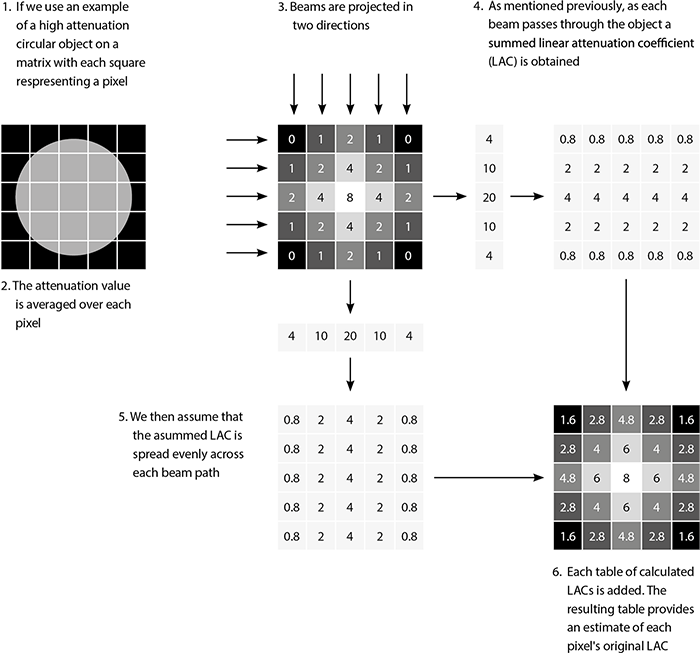
\includegraphics{CT_backprojection}
  \caption{An example of reconstruction with FBP using only 2
    projections
    \cite{abdulla2025acquiring2}.\label{fig:CT_reconstruction}}
\end{figure}

\begin{enumerate}
\item \textbf{Calibration}: A phantom patient (that we know exactly
  its morphology) is used to test if the reconstructions have some
  problem, such as for example, the detector sensitivity (affects to
  the contrast), ``dead-pixels'' in the detector (that should be
  interpolated), etc. This task should bezz performed periodically.
\item \textbf{Denoising}: The sinograms used to be quite
  smooth. Therefore, some technique for removing noise can be
  useful. This task is performed in every scan.
\item \textbf{Logarithmic transformation}: The X-rays are
  exponentially attenuated when they travel across the tissues. This
  step generates LACs (Linear Attenuation Coefficient), and allows to
  suppose that the rest of tasks are using linear data.
\item \textbf{Filtered BackProjection (FBP)}: A 3D reconstruction
  matrix accumulates in each voxel the constribution of each
  projection \cite{abdulla2025acquiring2} (see
  Figure~\ref{fig:CT_reconstruction})), that previously has been
  filtered using a high-pass filter to sharpen the textures of the
  reconstruction. Such filtering is usually performed in the Fourier
  domain, where the convolution is a linear-time
  operation.\footnote{The FFT (Fast Fourier Transform, both forward
    and inverse) is $\mathcal{O}(n\log_2(n))$ and the multiplication
    is $\mathcal{O}(n)$, where $n$ is the number of elements to
    convolve. Convolution in the signal domain is
    $\mathcal{O}(n^2)$. The sinograms must be FFT-transformed
    ($\mathcal{O}(n\log_2(n))$), perform the point-wise multiplication
    ($\mathcal{O}(n)$), and inverse FFT-transformed
    (($\mathcal{O}(n\log_2(n))$)). Therefore, for large enough $n$,
    convolution in the Fourier domain is faster.}

  Alternatively, instead of FBP an (usually ``heavier'') iterative
  reconstruction algorithm can be used.\footnote{These algorithms
    start with an initial guess of the image, calculate forward
    projections, compare them to the actual measured projection data
    to generate an "error matrix," and then use this error to update
    the image in successive iterations until an accurate depiction of
    the scanned object is achieved.}
  
  These algorithms start with an initial guess of the reconstruction
  (for example, using FBP). With this (possiblely unperfect)
  reconstruction all the sinograms are regenerated (simulating the
  real X-ray paths). By comparing the simulated sinograms and the
  originals, it is possible to determine which voxels of the
  reconstruction should be modified to make such comparison error
  small enough.

\end{enumerate}

\section{Quantum noise}

The processes by which radiation is emitted and interacts with matter
are inherently random, making all radiation measurements, including
medical imaging, subject to random error. The Poisson distribution is
particularly relevant to quantum noise in radiological imaging. The
noise per pixel ($\sigma$) is approximated by the square root of the
mean number of photons ($N$) recorded in each detector element, i.e.,
$\sigma = \sqrt{N}$ \cite{bushberg2011essential}.

In CT, quantum noise tends to dominate at high spatial frequencies in
the projection data, which can lead to unacceptably noisy
reconstructed images if appropriate filtering is not applied
\cite{bushberg2011essential}.

